\begin{figure}[htbp]
			\centering
			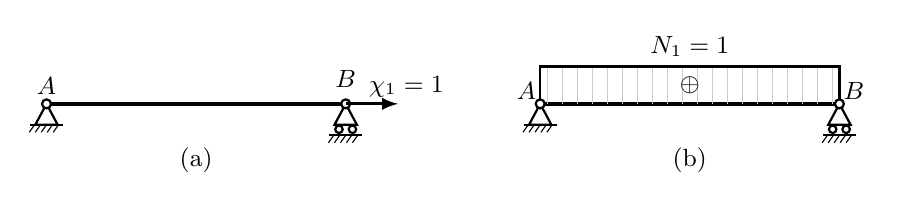
\begin{tikzpicture}[scale=0.95,>=latex,
				trave/.style={line width=1.2pt},
				forza/.style={black, line width=1pt},
				diagN/.style={black, line width=0.8pt},
				hatch/.style={gray!40, line width=0.3pt},
				]
				% ── Parametri ──
				\def\tw{0.15}\def\thR{0.28}\def\rn{0.06}
				\def\rw{0.05}\def\bw{0.09}\def\gw{0.22}\def\hh{0.10}
				\def\Lb{4}\def\hU{0.5}     % \hU = altezza del diagramma N1 (uniforme = 1)
				% ── Vincoli ──
				\def\cerniera#1{%
					\draw[thick] (#1,0) -- (#1-\tw,-\thR) -- (#1+\tw,-\thR) -- cycle;
					\draw[thick] (#1-\gw,-\thR) -- (#1+\gw,-\thR);
					\foreach \x in {-0.16,-0.08,0,0.08,0.16}
					\draw[thin] (#1+\x,-\thR) -- ++(-0.07,-\hh);
					\draw[thick, fill=white] (#1,0) circle (\rn);}
				\def\carrello#1{%
					\draw[thick] (#1,0) -- (#1-\tw,-\thR) -- (#1+\tw,-\thR) -- cycle;
					\draw[thick] (#1-\bw,-\thR-\rw-0.01) circle (\rw);
					\draw[thick] (#1+\bw,-\thR-\rw-0.01) circle (\rw);
					\draw[thick] (#1-\gw,-\thR-2*\rw-0.04) -- (#1+\gw,-\thR-2*\rw-0.04);
					\foreach \x in {-0.16,-0.08,0,0.08,0.16}
					\draw[thin] (#1+\x,-\thR-2*\rw-0.04) -- ++(-0.07,-\hh);
					\draw[thick, fill=white] (#1,0) circle (\rn);}
				
				% ===================== (a) sistema principale con la sola chi_1=1 =====================
				\begin{scope}[xshift=0cm]
					\draw[trave] (0,0) -- (\Lb,0);
					\cerniera{0}\carrello{\Lb}
					\node[above, font=\small] at (0,0) {$A$};
					\node[above=1pt, font=\small] at (\Lb,0.05) {$B$};
					\draw[->, forza] (\Lb,0) -- (\Lb+0.7,0);
					\node[above right=-1pt, font=\small] at (\Lb+0.22,0) {$\chi_1=1$};
					\node[font=\small] at (\Lb/2,-0.75) {(a)};
				\end{scope}
				
				% ===================== (b) diagramma N1 (uniforme, trazione, sopra l'asse) =====================
				\begin{scope}[xshift=6.6cm]
					\draw[trave] (0,0) -- (\Lb,0);
					\foreach \x in {0.1,0.3,...,3.9}\draw[hatch] (\x,0)--(\x,\hU);
					\draw[diagN] (0,0)--(0,\hU)--(\Lb,\hU)--(\Lb,0);
					\cerniera{0}\carrello{\Lb}
					\node[above left=-2pt, font=\small] at (0,0) {$A$};
					\node[above right=-2pt, font=\small] at (\Lb,0) {$B$};
					\node[font=\small] at (\Lb/2,0.5*\hU) {$\boldsymbol{\oplus}$};
					\node[above, font=\small] at (\Lb/2,\hU) {$N_1=1$};
					\node[font=\small] at (\Lb/2,-0.75) {(b)};
				\end{scope}
				
			\end{tikzpicture}
			\caption{a)~problema ``1'': forza iperstatica unitaria $\chi_1=1$ in $B$;
				b)~sforzo normale $N_1$, uniforme in trazione e pari a $1$.}
			\label{fig:stat_iper_long_01-p1}
		\end{figure}
